\documentclass[preprint,review,11pt,a4paper]{elsarticle}

\usepackage[hyperfootnotes=true]{hyperref}
\usepackage{amssymb}
\usepackage{algorithm}
\usepackage{amsmath}
\usepackage{array}
\usepackage{graphicx}
\usepackage{pifont}
\usepackage{tabularx,multirow,booktabs}
\usepackage{bm}
\usepackage[noend]{algpseudocode}
\usepackage{epsfig,subfigure}
\usepackage{mathptmx}
\usepackage{url}
\usepackage[marginal]{footmisc}

\journal{Neurocomputing}

\begin{document}

\begin{frontmatter}

% first the title is needed
\title{Distributed and Asynchronous Stochastic Gradient Descent with Variance Reduction}

%% Group authors per affiliation:
\author[mymainaddress]{Yuewei Ming\corref{mycorrespondingauthor}}
\cortext[mycorrespondingauthor]{Corresponding author}
\ead{ywming@nudt.edu.cn}

%% or include affiliations in footnotes:
\author[mymainaddress]{Yawei Zhao}
\author[mymainaddress]{Chengkun Wu}
\author[mymainaddress]{Kuan Li}
\author[mysecondaryaddress]{Jianping Yin}
\address[mymainaddress]{College of Computer,\\ National University of Defense Technology, Changsha 410073, China}
\address[mysecondaryaddress]{State Key Laboratory of High Performance Computing,\\ National University of Defense Technology, Changsha, 410073, China}

\begin{abstract}
Stochastic Gradient Descent (SGD) with variance reduction techniques has been proved powerful to train the parameters of various machine learning models. However, it cannot support the distributed systems trivially due to the intrinsic design.  Although conventional studies such as PetuumSGD perform well for distributed machine learning tasks, they mainly focus on the optimization of the communication protocol, which do not exploit the potential benefits of a specific machine learning algorithm. We analyze the asynchronous communication protocol in PetuumSGD, and propose a distributed version of variance reduced SGD named \emph{DisSVRG}. Specifically, DisSVRG adopts the variance reduction technique to update the parameters of a model. After that,  those newly learned parameters across nodes in a cluster are shared by using the asynchronous communication protocol. Besides, we accelerate DisSVRG by using the learning rate with an acceleration factor, and an adaptive sampling strategy is proposed in DisSVRG, which greatly reduces wait time during the iterations and speeds up the convergence of DisSVRG. Extensive empirical studies verify that DisSVRG  converges faster than the state-of-the-art variants of SGD, and gains almost linear speedup in a cluster.
\end{abstract}

\begin{keyword}
Stochastic gradient descent, Variance reduction, Asynchronous communication protocol, Distributed machine learning algorithms
\end{keyword}

\end{frontmatter}

\section{Introduction}
\label{introduction}

Machine learning based applications such as image recognition \cite{Coates2011An}, speech recognition \cite{dahl2012context} and text processing \cite{collobert2008unified} proliferate in the era of Big Data. Those underlying machine learning models are usually complex and big with a large number of parameters which can be trained or learned from a large amount of training data. For example, it is possible to train a large scale deep neural network which consists of millions or even billions of parameters by feeding it with terabytes of training data. Furthermore, it is worth noting that most of the machine learning algorithms are iteratively convergent, which means those algorithms need many rounds of iterative calculations to update the parameters of their models. Considering the complexity of the underlying model, the huge size of the training data and the massive amount of computation, an efficient training method is vitally important for performing a large scale learning task.

Many machine learning algorithms can be described by the optimization problem like (\ref{equa_loss_minimization}),
\begin{equation}
\label{equa_loss_minimization}
\min f(\omega),~~~~~f(\omega)=\frac{1}{n}\sum\limits_{i=1}^n f_i(\omega) + R(\omega).
\end{equation}  Here, $\nabla$ stands for the derivation operation. $f(\omega)$ is generally called the loss function.  $\omega$ represents the parameters of a model, that is, the parameters needed to be updated during the iterations. $n$ means the size of training data. $R(\omega)$ represents the regularization item which is used to avoid overfitting. The regularization item represents the prior knowledge about the problem. For example, when we want to obtain a sparse solution, that is, the optimal parameters contain many zeros, $R(\omega)$ is usually formulated as $L_1$ norm, namely, $R(\omega) = \lVert \omega \rVert_1$. Besides, ridge regression modes use the $L_2$ norm as the regularization item, that is, $R(\omega) = \lVert \omega \rVert_2$. Some other regularizations can be used in the optimization objective \cite{Vidaurre:2013cu, Gnecco2015Learning, Cucker2002On}, but it is out of the scope of the paper. We recommend readers to read those references for more details. 

The loss function $f(\omega)$ can be minimized by updating the parameters iteratively, which is called the learning process. Conventionally, the gradient descent method is used to compute the global average gradient, i.e., $\nabla f(\omega_{t-1})$, and then uses it to update the parameters during an iteration. Here, $t$ represents the $t$th iteration. Since $\nabla f(\omega_{t-1})$ needs $n$ derivations, which are time-consuming, the gradient descent method is not practical for a large scale learning task.  An alternative approach  is Stochastic  Gradient Descent (SGD) and its variants. SGD randomly samples an instance from the training data, and then use it to compute the local gradient, i.e., $\nabla f_i(\omega_{t-1})$, instead of the global average gradient.   The parameters are thus updated by using the local gradient. Since $\nabla f_i(\omega_{t-1})$ merely needs one derivation for the local gradient during an iteration,  it is efficient for the large scale learning tasks.  However, since $f_i$ is randomly sampled, the variance exists between the local gradient $\nabla f_i(\omega_{t-1})$ and the global average gradient $\nabla f(\omega_{t-1})$, which slows the convergence of the loss function i.e., $f(\omega)$, of a machine learning algorithm.  Specifically, when the parameters are close to the optimal state, it is difficult to decrease the loss function due to the variance. Conventionally, the variance is reduced by using a decaying learning rate to update the parameters. That is,  the value of the learning rate is decreased when the iteration proceeds. Although the variance can be reduced by the decaying learning rate, the small learning rate unavoidably  leads to the slow convergence.


Recently, the SGD and its variants have been widely used to train the parameters of a model in distributed memory systems \cite{Dean:2012wx, Li:2014tt, Xing:2015ib}. Those versions of SGD generally train and update parameters in a parameter-server system by using a cluster. The nodes in the parameter-server system are categorized into servers and workers. The underlying calculations of the gradients are conducted by workers. Those updates will be then pushed to servers, and be aggregated on servers for updating the global parameters. Finally, those newly learned global parameters will be shared with workers. Since there exists much communication between workers and servers, all the distributed versions of SGD like PetuumSGD focus on the optimization of communication \cite{Xing:2015ib}.  In specific, PetuumSGD has proposed the asynchronous communication protocol denoted by Staleness Synchronous Protocol (SSP) to conduct communication across nodes. SSP outperforms the Bulk Synchronous Protocol (BSP) employed on Hadoop or Spark significantly. However, since SSP is designed for the general iteratively convergent machine learning algorithms, it does not exploit the potential benefits of SGD to accelerate the iterative calculations. For example, PetuumSGD updates the parameters by using a decaying learning rate. The learning rate in PetuumSGD in the current iteration denoted by $\eta$ will become $0.95\eta$ in the next iteration. When the parameters are close to the optimal state, the loss function is difficult to be decreased due to the extremely small learning rate. In a nutshell,   even though PetuumSGD adopts SSP  to optimize the communication between workers and servers, the decay learning rate slows the convergence.

Meanwhile, a new technique of the variance reduction is proposed to speed up the convergence of SGD \cite{Johnson:9MAvkbgy, Zhao:SZfxEHHg, Reddi:2015vj}. Such variance reduction technique reduces the variance of SGD, and keeps SGD converging at a constant rate.   However, those versions of SGD are designed to be used in one node instead of a cluster. When the amount of parameters or the size of training data is extremely huge so that they cannot be stored in a node, the underlying variance reduction technique will not work. For instance, a deep network may have billions or even trillions of parameters, which cannot be stored in a node. Therefore, such versions of SGD are incapable of performing the training for a large scale learning task, or handling a large amount of training data.

In this paper, we design a distributed and asynchronous version of variance reduced SGD denoted by DisSVRG for large-scale machine learning tasks. It is worth noting that DisSVRG adopts the asynchronous communication protocol, i.e., Staleness Synchronous Protocol (SSP). In order to obtain a fast convergence, DisSVRG is accelerated by using a learning rate with an acceleration factor. It is unavoidable that the fast workers will spend much time on waiting for the slow workers when performing iterative calculations  in a cluster, which is also known as the "straggler problem". The straggler problem wastes much time for the fast workers, thus leads to the slow convergence of a machine learning algorithm. In order to reduce the wait time, we propose an adaptive sampling strategy to alleviate the straggler problem. Specifically, we dynamically adjust the random sampling strategy during the iterations. When the worker is faster than other workers, it will  sample more instances for the next iteration, which will take the faster worker more time to compute the local gradient.   Thus, the slow workers have chance to catch up with the faster works, and  the wait time is reduced significantly. Finally, we conduct empirical studies on the HPC cluster of the \emph{Tianhe-1} supercomputer which is located in the National Supercomputing Center in Changsha. The performance evaluation verifies that DisSVRG outperforms the state-of-the-art version of SGD, and obtains approximately linear speedup in the cluster.


The rest of this paper is organized as follows. Section \ref{related_work} outlines the related work. Section \ref{sect_preliminary} presents the preliminaries of our method. Section \ref{implementation} illustrates the details of DisSVRG. Section \ref{optimization_sgd} highlights the  optimization of DisSVRG. Section \ref{discussion} discusses the major difference between our work and the previous studies. Section \ref{performance_evaluation} shows the performance evaluation. Section \ref{conclusion} concludes the paper.


\section{Related work}
\label{related_work}

%\subsection{Asynchronous distributed stochastic gradient descent}
With the proliferation of data, a complex and big model can be learned by feeding it with a huge size of training data. An approach for such a large scale learning is to use a cluster to train the parameters of the underlying model \cite{Dean:2012wx, Li:2014tt, Xing:2015ib}. Dean et al. propose a version of asynchronous and distributed SGD denoted by \emph{DownpourSGD} in a parameter server system. DownpourSGD uses fully asynchronous communication protocol to conduct communication across nodes, which cannot guarantee the convergence. To increase the robustness of DownpourSGD, the Adagrad adaptive learning rate procedure is adopted \cite{Cavalcante:2009il}. However, the adopted learning rate is decayed with the iterations, and thus leads to the slow convergence. Besides, Li et al. and Xing et al. have proposed an implementation of the parameter server system, respectively.  The similar asynchronous communication protocol denoted by SSP is adopted in both of their systems to share the updates of the parameters across nodes. SSP has been proved powerful in both theory and practice.  However, SGD in \cite{Li:2014tt} uses a constant learning rate without variance reduction technique, leading to slow convergence due to the variance. SGD in \cite{Xing:2015ib}, i.e., PetuumSGD, adopts a decaying learning rate to reduce the variance, giving rise to slow convergence when the learning rate becomes small. Our version of the asynchronous and distributed SGD, i.e., DisSVRG, adopts SSP to implement the communication across nodes, and uses the variance reduction technique  to reduce variance as well. Recently, Zhang et al. have proposed a new distributed variant of SGD denoted by SSGD in the paper \cite{Zhang:2015tp}.  SSGD is designed by combining the delayed proximal gradient and the stochastic variance reduced gradient. Although SSGD outperforms other previous variants of SGD because of the variance reduction technique, our proposed method DisSVRG has an advantage of the convergence performance over it. Additionally, there are some other impressive researches about the distributed machine learning in a cluster. For example, Aaron et al. focus on the straggler problem in the distributed settings, and propose FlexRR to solve the problem for iteratively convergent machine learning algorithms \cite{Harlap:2016ia}.  Li et al. propose an efficient mini-batch training mechanism to accelerate SGD in a cluster  \cite{Li:2014jg}. 



%\subsection{Asynchronous parallel stochastic gradient descent with variance reduction technique}
The variance reduced SGD denoted by \emph{SVRG} is adopted in \cite{Johnson:9MAvkbgy}, which is  effective to reduce the variance of SGD. However, SVRG is a serial version, and designed to be run on a single node. Thus, it is not suitable for a large scale learning task. Asynchronous and parallel versions of SVRG partially solve this problem \cite{Zhao:SZfxEHHg, Reddi:2015vj, Mania:2015wa, lian2015asynchronous, Pan:2016wx}. Such SVRG versions use the lock-free method to update the parameters in parallel for multiple learning threads in a node. However, the design of such work targets at a multicore system on a single node. When the size of training data or the number of parameters  is huge so that they can not be stored in one node, SVRG and those variants fail immediately. Our proposed variance reduced SGD is designed for  the large scale learning tasks in a cluster. We can partition the data into multiple blocks, and allocate them to multiple worker machines, which is suitable to accelerate SGD in a cluster. More recently, there are many new variants of the variance reduced SGD such as SAGA \cite{Defazio:2014vu}, S2GD \cite{Richtarik:2013te}, SVRG++ \cite{Allen2015Improved}, Prox-SVRG \cite{Xiao:2014vw}. Those great researches have proposed advanced variance reduction techniques, which can be used to improve our method. However, it is out of the scope of the paper, and we leave it as the future work.


\section{Preliminaries}
\label{sect_preliminary}
In this section, we present the preliminaries including the parameter server system and the data parallelism, and the variance reduced SGD.
\subsection{Parameter server and data parallelism}
\label{parameter server}

In data-parallel machine learning, the data set $D$ is partitioned into $P$ blocks. The blocks of data are assigned to the worker machines which are indexed by $p=1, \ldots, P$. We denote the $p$th data block by $D_p$. The data parallelism updates the model parameters as follows:
\begin{equation}
\omega^s=G\left(\omega^{s-1}, \sum_{p=1}^P\Delta(\omega^{s-1}, D_p)\right).
\end{equation} Here, $\Delta(\cdot)$ means the update of the parameters which is obtained according to the data partition $D_p$ on a worker. In specific, the worker needs to pull the initial parameters from the model server. After that, it computes the update of the parameters, i.e. $\Delta(\omega^{s-1}, D_p)$. $G(\cdot)$ represents the aggregation of the updates of the parameters on a server. Specifically, the server collects all the updates from the workers, and then conduct the aggregation \cite{ho2013more} \cite{xing2015petuum}. Taking SGD as an example, the update rule can be
\begin{equation}
\omega^s=\omega^{s-1} + \sum_{p=1}^P\eta \Delta(\omega^{s-1}, D_p),
\end{equation}
where $G(\cdot)$ is initialized as an additive operation, and $\Delta(\omega^{s-1}, D_p)$ is usually initialized  as the product of the learning rate $\eta$ and the gradient according to the data partition $D_p$. As shown in Figure \ref{figure_data_parallelism},  servers and workers interact via a bipartite topology. The model parameters $\omega$ can be divided and stored on multiple servers and thus not limited by a single machine's memory in a parameter server system. Every worker pulls the parameters from the server, and then  obtain the update of the parameters. Finally, those updates are pushed to the servers, and are aggregated on those servers. The servers can collaborate with the workers to utilize CPUs on all machines when we conduct a large scale machine learning task \cite{dai2015high} \cite{ho2013more}.

\begin{figure*}
\centering
\label{figure_data_parallelism}
\subfigure{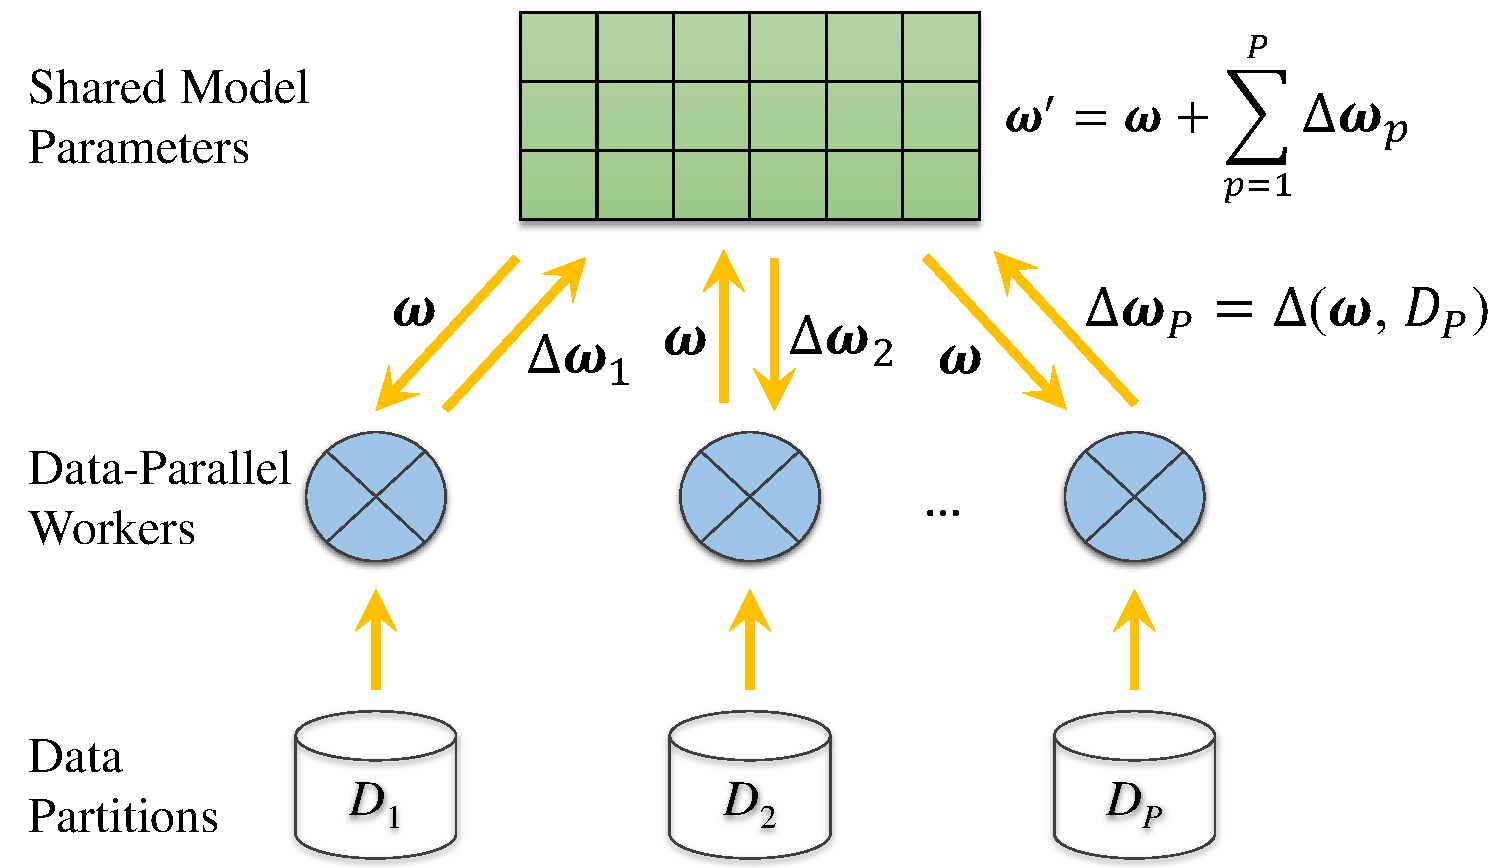
\includegraphics[width=0.49\columnwidth]{figures/data_parallelism_on_PS}\label{figure_data_parallelism_on_PS}}
\subfigure{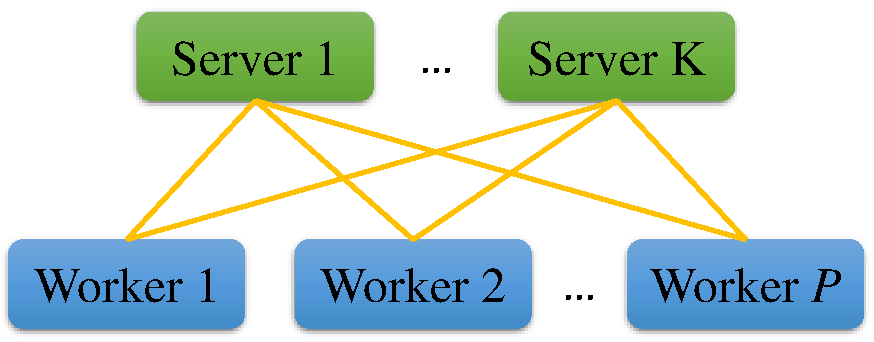
\includegraphics[width=0.49\columnwidth]{figures/PS_topology}\label{figure_PS_topology}}
\caption{Illustration of data parallelism and Parameter Server topology}
\end{figure*}


\subsection{Variance reduced SGD}
The variance reduced SGD uses a variance reduced gradient to reduce the stochastic noise during the update of the parameter. The variance reduced gradient is formulated as 
\begin{equation}
\label{equa_vr_gradient}
\begin{array}{ll}
\nu_t = \nabla f_{i_t} - \nabla \tilde{f}_{i_t} + \nabla \tilde{f}.
\end{array}
\end{equation} Here, $i_t$ represents the index of an instance which is picked at the $t$th iteration. $\nabla f_{i_t}$ represents the stochastic gradient, $\nabla \tilde{f}_{i_t}$ represents the noise reducer, and $\nabla \tilde{f}$ represents  the stale full gradient. First, $\nabla f_{i_t}$ usually leads to much stochastic noise because of it is different from the full gradient. The stochastic noise is denoted by variance in the paper. Compared to the gradient descent, the convergence of the SGD is a  victim of the variance, and usually converges slowly. To overcome the weakness of the SGD, the variance gradient uses $\nabla \tilde{f}_{i_t}$ and  $\nabla \tilde{f}$ to reduce the variance due to the following property:
\begin{equation}
\label{equa_vr_gradient}
\begin{array}{ll}
\mathbb{E}\nu_t = \mathbb{E}(\nabla f_{i_t} - \nabla \tilde{f}_{i_t} + \nabla \tilde{f}) = \nabla f.
\end{array}
\end{equation} That is to say, the variance reduced gradient is equivalent to the full gradient at every iteration in expectation. It is worthy noting that $\nabla \tilde{f}$ is a stale full gradient, which is updated at the start of an epoch and kept fixed during the iterations in an epoch.  Therefore, the variance reduced gradient reduces the stochastic noise significantly, but leads to less computational cost. Extensive empirical studies show that the variance reduced gradient leads to the comparable computational cost of SGD, but obtains the equivalent convergence performance of gradient descent.



\section{System implementation}
\label{implementation}
In the section, we present the details of the system implementation including the algorithm and the distributed mechnism.
\subsection{Overview}
Our distributed and asynchronous SGD denoted by DisSVRG is presented  in Algorithm \ref{algorithm_dis_svrg}. DisSVRG consists of three ingredients: the epochs of iterations (the outer \emph{for} loop at Line 2), the random sampling strategy of the training data (the inner \emph{for} loop at Line 6) and the update rule of the parameters (Lines 8-9). DisSVRG is launched by the servers, and all the workers will be informed by message passing. Once a worker receives the message from a server, it pulls a copy of the global parameters from a server, and  begins conducting the calculations during the epoch. The random sampling strategy is conducted by the workers. When a worker randomly samples an instance from the training data, it computes the variance reduced gradient (Line 8), and updates the local parameters with the local gradient (Line 9). When the local parameters have been updated, the newly learned parameters will be sent to a server. The inter-node communication is conducted by the asynchronous communication protocol, i.e., SSP. The server receives these learned parameters  and aggregates them. The aggregated parameters are the latest global parameters which will be sent to workers for the next iteration. The details of communication across nodes and aggregation of parameters will be demonstrated in Section \ref{implementation}.

\begin{algorithm}[t]
    \caption{DisSVRG}
    \label{algorithm_dis_svrg}
    \begin{algorithmic}[1]
        \State Initialize $\tilde{\omega}^0$. $ \verb|\\|$ Pull the global parameters by all workers from the servers.
        \For {$s=1,2,...$} $ \verb|\\|$ Asynchronously update the parameters by all workers.
            \State $\tilde{\omega}=\tilde{\omega}^{s-1}$.
            \State $\tilde{f}(\tilde{\omega})=\frac{1}{n}\sum\limits_{i=1}^n\nabla f_i(\tilde{\omega})$.
            \State $\omega_0=\tilde{\omega}$.
            \For {$t=1,2,..., m$}
                \State randomly sample $i_t\in\{0,1,2,...,m\}$.
                \State $v_t=\nabla f_{i_t}(\omega_{t-1})-\nabla f_{i_t}(\tilde{\omega})+\tilde{f}(\tilde{\omega})$. $ \verb|\\|$Variance reduced gradient.
                \State $\omega_t=\omega_{t-1}-\eta v_t$. $ \verb|\\|$Update the parameters with variance reduction gradient.
           \EndFor
           \State $\tilde{\omega}^s=\omega_m$. $ \verb|\\|$Push the newly learned parameters to the servers, and aggregate them with the global parameters.
       \EndFor
    \end{algorithmic}
\end{algorithm}

\subsection{Distributed implementation}
DisSVRG is designed for the distributed memory systems where the nodes can be categorized into workers and servers. Every worker caches a copy of the parameters which is called the \emph{local parameters}; while all the servers maintain one copy of the parameters which are called the \emph{global parameters}. The global parameters will be pulled by a worker and be used as the initial parameters for an iteration. Meanwhile, such initial parameters will replace the stale local parameters on the worker and become its new local parameters.

\textbf{Server:}    The servers control the iterations by using the asynchronous communication protocol, i.e., SSP.  Since the runtime environment of nodes in a cluster varies a lot, the  time overhead of an epoch for different workers  varies. Therefore, there are fast and slow workers which conduct an epoch fast and slow respectively.   It is worth noting that DisSVRG may not converge if all the workers update parameters in a fully asynchronous way. Therefore, we set a delay bound, i.e., $\tau$. The delay $\tau$ is used to synchronize all the workers. For instance, when the fastest worker finishes the $t$th iteration, and the slowest worker does not finish the $(t-\tau)$th iteration, the fastest worker will be forced to stop and wait for the slowest one. In specific, the fastest worker can not  pull a copy of the global parameters from the servers, and thus has to wait for the slowest worker. Until the slowest worker finishes the $(t-\tau)$th iteration, the fastest worker will re-start to conduct the iterations. When a server receives the newly learned parameters from a worker, it will aggregate them with the global parameters on the server. After that, the latest parameters on the server will be pulled by the worker for the next iteration.
The details are illustrated in Algorithm \ref{algorithm_dis_svrg_server}.

\begin{algorithm}[t]
    \caption{Server}
    \label{algorithm_dis_svrg_server}
    \begin{algorithmic}[1]
        \State Initialize $\tilde{\omega}^0$.
        \While {true}
            \If {receive a pull request from the worker $p$.}
               \State $e_p=p.epoch$.
                \If {all the workers have finished $(e_p-\tau)$th epoch.}
                    \State send a copy of the global parameters to the worker $p$.
                \EndIf
            \EndIf
            \If {receive a push request from the worker $p$.}
                \State receive the newly learned parameters from the worker $p$.
                \State aggregate the newly learned parameters with the global parameters on the server.
            \EndIf
        \EndWhile
    \end{algorithmic}
\end{algorithm}

\textbf{Worker:} Workers in a cluster conduct machine learning tasks in asynchronous way. They pull the parameters from the servers by message passing. If a  copy of the global parameters is pulled to the workers, those workers begin iterative calculations. During an epoch, workers first randomly pick an instance from the training data, then use the instance to compute the gradient.  All the workers are independent with peers when conducting iterative calculations. When an epoch is finished, a worker has learned the new parameters, and will send those newly learned parameters to a server. It is the servers that control when to synchronize among the workers.

\begin{algorithm}[t]
    \caption{Worker}
    \label{algorithm_dis_svrg_worker}
    \begin{algorithmic}[1]
        \While{true}
            \State send a pull reworkerquest to a server.
            \While {true}
                \If {receive a copy of the global parameters from the server.}
                    \State cache it as the new local parameters, i.e., $\tilde{\omega}$.
                    \State $\nabla \tilde{f}(\tilde{\omega})=\frac{1}{n}\sum\limits_{i=1}^n\nabla f_i(\tilde{\omega})$.
                    \For {$t=0,1,2,..., m$}
                       \State randomly sample a non-negative number $i$ with $i\in\{0,1, 2,...,n\}$.
	              \State $v_t=\nabla f_{i_t}(\omega_{t-1})-\nabla f_{i_t}(\tilde{\omega})+\nabla \tilde{f}(\tilde{\omega})$.
	              \State $\omega_t=\omega_{t-1}-\eta v_t$.
                    \EndFor
                    \State send  $\omega_m$ to a server.
               \EndIf
        \EndWhile
      \EndWhile
    \end{algorithmic}
\end{algorithm}

\textbf{Aggregation:} When the workers push their newly learned parameters to the servers, those parameters will be aggregated with the global parameters on the servers. The average between the newly learned parameters and the global parameters will be identified as the latest global parameters, and will wait to be pushed to all the workers for the next iteration.

\textbf{Update rule:} As illustrated in Algorithm \ref{algorithm_dis_svrg_worker}, DisSVRG is significantly different from the standard SGD because of the variance reduction technique. In the standard SGD, the update rule is shown as follows.
\begin{equation}
\label{standard_sgd}
v_t=\nabla f_{i_t}(\omega_{t-1})
\end{equation}

$v_t$ in the standard SGD is not the global gradient, which leads to variance, and slows the convergence of the loss function unavoidably. Instead, the variance reduction technique is used in DisSVRG effectively reduce the variance \cite{Johnson:9MAvkbgy}. Considering the $i$th round of the iterations, since $i_t$ is randomly picked, it holds that
\begin{equation}
\mathbb{E}\nabla f_{i_t}(\omega_{t-1})=\nabla f(\omega_{t-1}),
\end{equation}
and
\begin{equation}
\mathbb{E}(-\nabla f_{i_t}(\tilde{\omega})+ \nabla \tilde{f}(\tilde{\omega}))= - \nabla \tilde{f}(\tilde{\omega})+\nabla \tilde{f}(\tilde{\omega})=0.
\end{equation}
Therefore,
\begin{equation}
\mathbb{E}( \nu_t )= \mathbb{E}(\nabla f_{i_t}(\omega_{t-1})-\nabla f_{i_t}(\tilde{\omega})+\tilde{f}(\omega))=\mathbb{E}(\nabla f_{i_t}(\omega_{t-1}))=\frac{1}{n}\nabla f(\omega_{t-1}).
\end{equation}
It is obvious that the variance of DisSVRG is reduced as expected. Unlike PetuumSGD and DownpourSGD, DisSVRG can converge fast without decaying the learning rate during the iterations. Benefiting from the variance reduction technique, DisSVRG  can converge at a constant rate.

\section{Optimization of DisSVRG}
\label{optimization_sgd}
In the section, we optimize the proposed method DisSVRG by adopting an adaptive learning rate and sampling strategy.

\subsection{Learning rate with an acceleration factor}
Generally, variance reduction technique accelerates machine learning algorithms by using a constant learning rate. Even though the constant learning rate performs well for $L$-smooth and $\gamma$-strongly convex objection function, some intrinsic properties can be exploited to accelerate the convergence of the machine learning algorithms.

We introduce an acceleration factor $\sigma$ with $\sigma=\parallel \nabla f_i(\omega)\parallel$ to the learning rate of DisSVRG. That is,
\begin{equation}
\eta=\eta_0+\sigma,~~~~~~\sigma=\parallel \nabla f_i(\omega)\parallel.
\end{equation}
The learning rate of DisSVRG contains two ingredients: the constant and the acceleration factor. The constant part of the learning rate get the parameters out of the local optimal state; while the acceleration factor speedup the convergence of DisSVRG. This setting of the acceleration factor is reasonable for the following reasons. First, the acceleration factor will become large when the parameters are far from the optimal state. If so, DisSVRG will converge fast accordingly. Second, the acceleration factor will not become so large that DisSVRG do not converge. Considering that the convex function $f_i$ in the machine learning model is $L$-smooth, $\nabla f_i$ will not be changed out of  a range for an iteration. That is, $\parallel\nabla f_i\parallel<C$. Here, $C$ is a non-negative constant. Third, when the parameters are close to the global optimal state, the acceleration factor $\sigma$ will become close to zero. DisSVRG thus almost converges to the global optimal state at a constant rate just like the original design in \cite{Johnson:9MAvkbgy}.

As illustrated in Fig. \ref{figure_evaluation_accelerated_factor}, we use the acceleration factor to conduct the linear regression tasks. Here, the evaluation test is conducted on a node instead of a cluster. The dataset is \emph{YearPredictionMSD} which is the largest dataset we can find to conduct linear regression tasks. Other settings of the evaluation are presented in Section \ref{performance_evaluation}.  We can get two important observations from Fig. \ref{figure_evaluation_accelerated_factor}. First, the learning rate with an acceleration factor makes the underlying machine learning algorithm converge faster than the constant learning rate without the acceleration factor. Second, the benefits become significant with a small basic learning rate. Shortly, the acceleration factor gives rise to obvious benefits to accelerate the convergence of a machine learning algorithm.

\begin{figure}
\centering
\subfigure{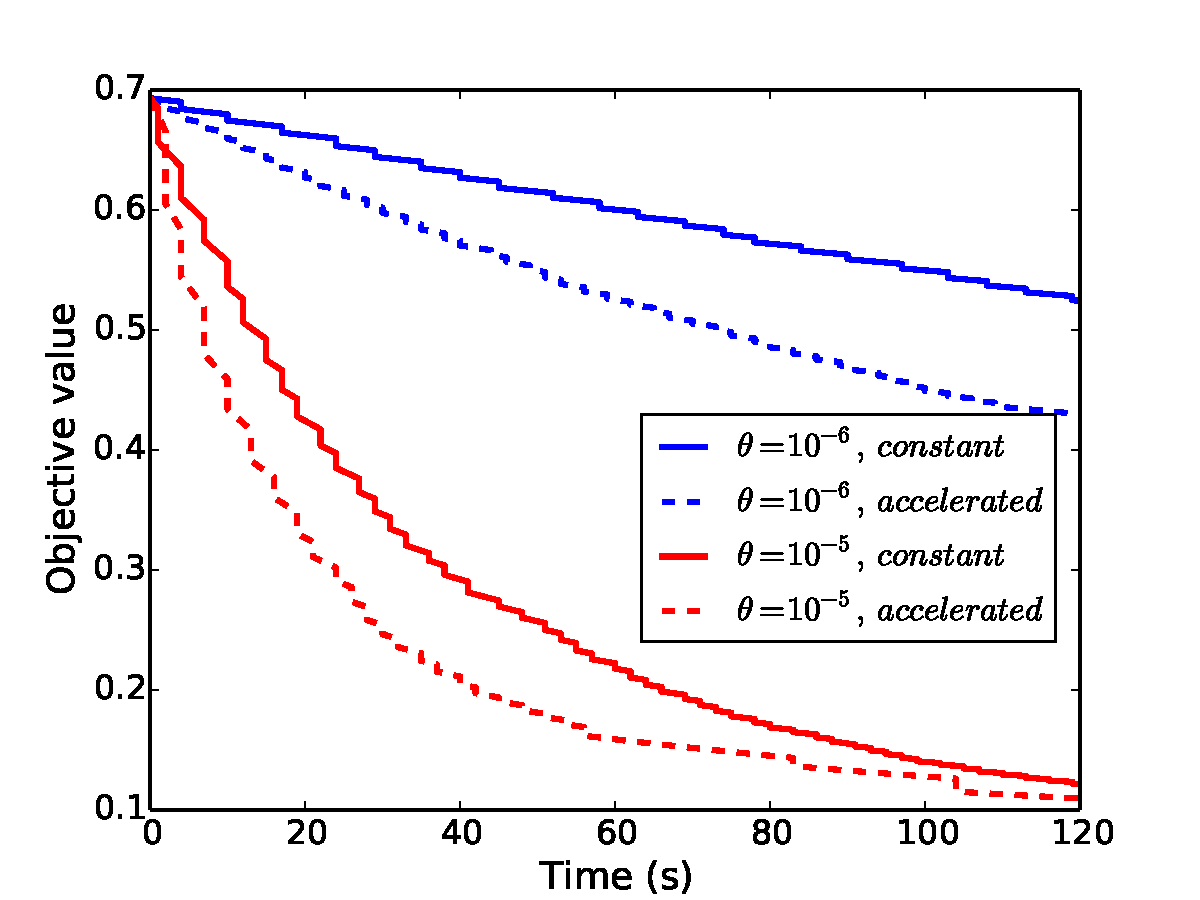
\includegraphics[width=0.50\columnwidth]{figures/evaluation_accelerated_factor}}
\caption{The learning rate with the acceleration factor makes DisSVRG converge fast significantly.}
\label{figure_evaluation_accelerated_factor}
\end{figure}

\subsection{Adaptive sampling strategy}

Since DisSVRG needs the sampling strategy to update the parameters during an epoch, it is important to identify how many random updates in an epoch are appropriate.  As illustrated in Algorithm \ref{algorithm_dis_svrg}, $m$ represents the number of updates for an epoch. First, $m$ cannot be given an extremely large number, which takes much time to update the local parameters during an epoch on a worker.  Second, $m$ cannot be set a small value straightly. If so, DisSVRG has to conduct many epochs to reduce the value of the loss function. Considering that the average gradient of the loss function is needed to conduct an epoch, a small $m$ means much computation of the average gradients, which is time-consuming.
%Therefore, it is important to find a good sampling strategy by identifying an appropriate $m$.
Additionally, it is worth noting that the workers in a cluster perform asynchronously due to the diversity of the runtime environment or the hardware in the heterogenous cluster.  Although the asynchronous communication protocol, i.e., SSP, allows a delay bound to relax the synchronization among the workers, those fast workers have to wait for the slow peers when the delay is met. Such wait time impairs the convergence of DisSVRG. An approach to reduce the underlying wait time is to adjust the sampling strategy dynamically.  Intuitively, the fast workers in the cluster should sample more instances during an epoch than the slow workers. That is, $m$ in the fast workers should be larger than that in the slow workers.

We adopt an adaptive dynamic sampling strategy which dynamically adjust $m$. When an epoch is completed, the newly learned local parameters will be pushed to a server. The server will check the epochs of the worker. If the worker is too fast, it needs to wait for other slow peers.  The fast workers will adjust  $m$ to be a large value, i.e., $m+\delta$. Here, $\delta$ is a non-negative integer with $\delta=0.05m$ in DisSVRG. By using this adaptive strategy, the fast workers will sample more instances during an epoch, thus spend more time on computing the updates of parameters than the slow workers. The slow workers have chance to catch up with the fast workers. Therefore, the wait time is reduced as a result. This adaptive sampling strategy has many benefits. The most important benefit is that the fast workers reduce the wait time, and use it  to converge DisSVRG. We conduct an evaluation test on a  node by varying the value of $m$. Here, the dataset is still \emph{YearPredictionMSD}, and the learning rate, i.e., $\eta$ is set to be a constant with $\eta=10^{-5}$. As illustrated in Fig. \ref{figure_evaluation_random_strategy_accelerated_factor},  it is obvious that a large $m$ brings a fast convergence of the objective function. Therefore, a large $m$ benefits to decrease the value of the loss function. Additionally, the wait time is compared in a cluster which consists of $5$ nodes.   As shown in Fig. \ref{figure_evaluation_random_strategy_wait_time}, the average wait time has been evaluated by varying $m$. Here, the delay is set to be $0$.  It is obvious that the adaptive sampling strategy  decreases the average wait time during iterations, and thus spend much time to accelerate the convergence of DisSVRG in reverse.

\begin{figure*}
\centering
\subfigure[]{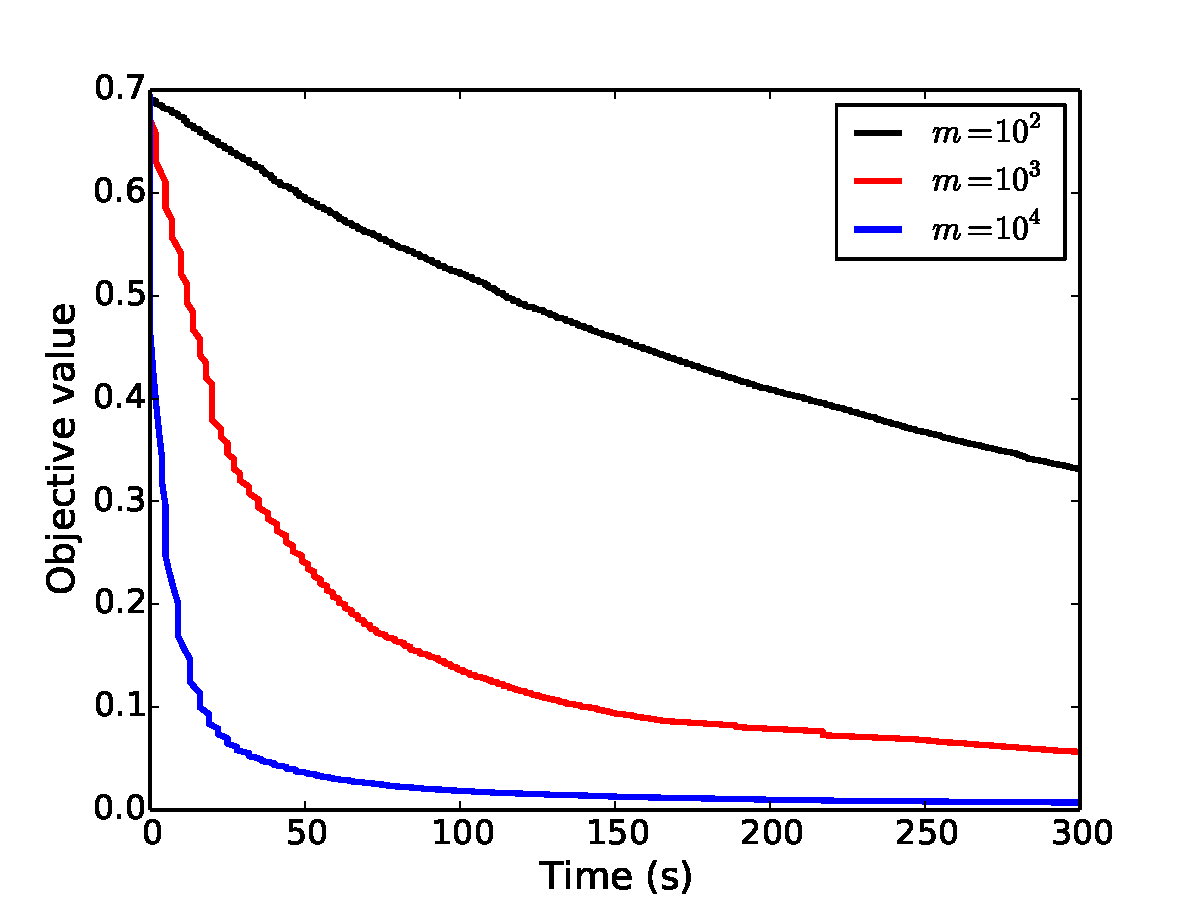
\includegraphics[width=0.49\columnwidth]{figures/evaluation_random_strategy}\label{figure_evaluation_random_strategy_accelerated_factor}}
\subfigure[]{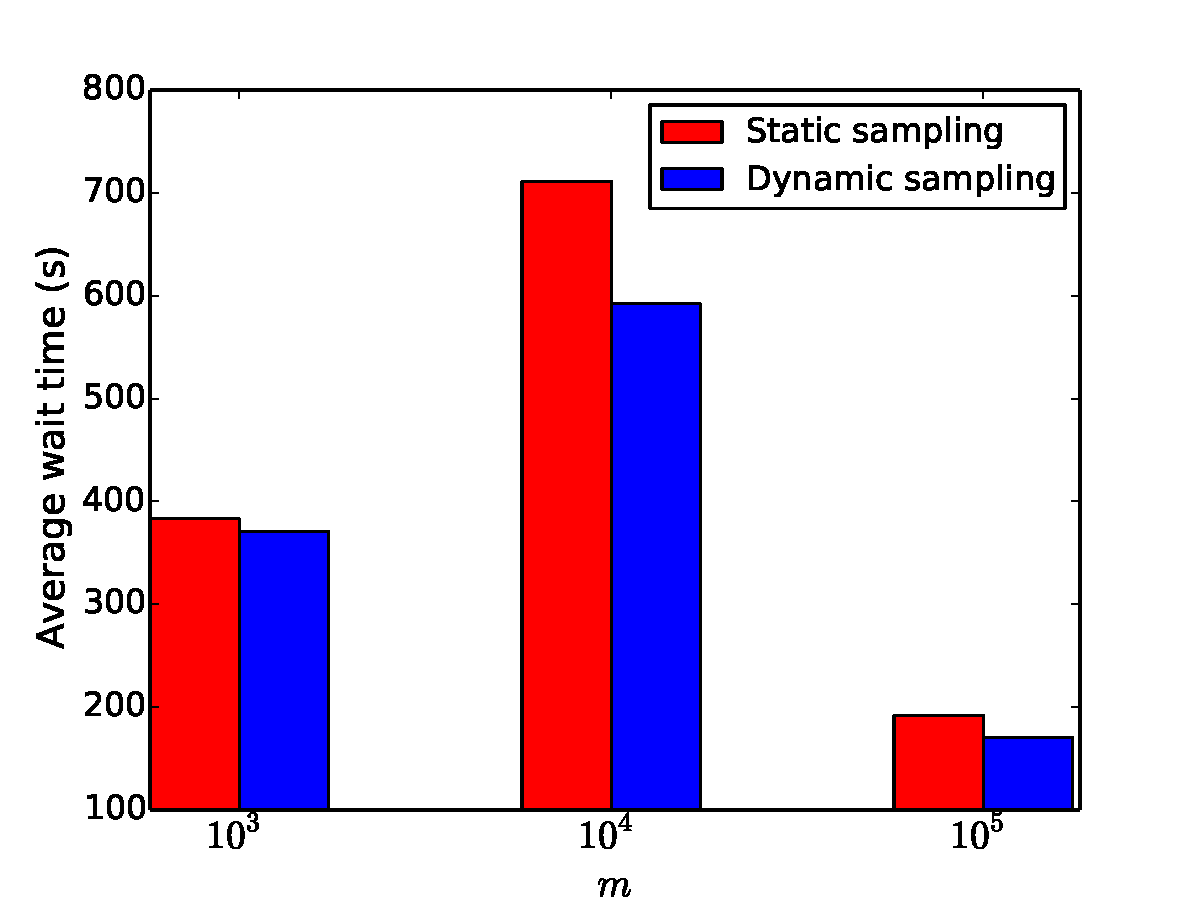
\includegraphics[width=0.49\columnwidth]{figures/evaluation_random_strategy_wait_time}\label{figure_evaluation_random_strategy_wait_time}}
\caption{A large $m$ leads to a fast convergence for DisSVRG, and reduces much wait time during iterations.}
\label{figure_evaluation_random_strategy}
\end{figure*}

\section{Discussion}
\label{discussion}
The machine learning tasks such as deep learning are generally fed with an extremely large volume of training data. However, conventional serial versions of SGD  cannot handle a huge training data on a single node within the available time. Although some distributed machine learning systems such as Petuum \cite{Xing:2015ib} and DMTK\cite{Yuan:2015ka} have been designed to solve this problem, those variants of SGD have their inner weakness, namely the variance. Such those distributed machine learning systems thus decrease the learning rate to reduce the variance, which leads to slow convergence of SGD. We do not aim to propose another a general platform for distributed machine learning algorithms, but focus on the optimization of SGD in a distributed system. Our implementation of the distributed SGD, i.e., DisSVRG, adopts the variance reduction technique to reduce the variance. Such variance reduction technique is the most difference between DisSVRG and PetummSGD. Although PetuumSGD  adopts a decaying learning rate, it slows to converge the loss function. DisSVRG has been accelerated with two ingredients: the constant and the acceleration factor. The constant factor is effective to get DisSVRG out of the local optimal state, and keeps converge at a constant rate. The acceleration factor will speedup the convergence of the machine learning algorithm. Even though DisSVRG adopts the same asynchronous communication protocol with PetuumSGD, it converges faster than PetuumSGD by adopting the powerful variance reduction technique.

DisSVRG improves SVRG with at least three aspects. First, we extend the serial SVRG to an asynchronous and distributed version by using the asynchronous consistency protocol, i.e., SSP. Second, comparing with the constant learning rate in SVRG, the learning rate in our SGD contains an acceleration factor which exploits the potential benefits of the loss function, and makes the machine learning algorithms converge fast. Third, SVRG needs to sample $m$ instances randomly to update parameters. SVRG sets $m$ multiple times of the size of training data, which is not practical for a large volume of training data. Instead, DisSVRG adopts an adaptive sampling strategy which adjusts the value of $m$ by the runtime environment of the worker dynamically. Specifically, the fast workers will sample more instances during the next epoch than the slow peers. The slow workers thus have chance to catch up with the fast workers. Thus, wait time is reduced significantly, which makes DisSVRG converge fast in the end. In a nutshell, considering the diversity of the runtime environment and the hardware in a cluster, DisSVRG is suitable to the practical scenarios.

Additionally, comparing with the version of SGD in \cite{Zhang:2015tp} denoted by \emph{SSGD}, our SGD adopts a more natural way to implement the distributed SGD with the variance reduction. SSGD implements the $\tau$-delay bound inconsistent protocol within an epoch, but keeps fully consistent protocol among different workers. Therefore, SGD in \cite{Zhang:2015tp} has at least two weaknesses. First, the fully consistency protocol for the workers is not suitable to the iterative convergence machine learning tasks \cite{2015_dai_high_performance_ml, Li:2014uy, Dai:2013vj}. Since the straggler problem usually exists among workers due to the variety of the system runtime environment or the hardware in the heterogenous cluster, the fast workers in \cite{Zhang:2015tp} have to wait for the slow workers, and start the next iteration in a synchronous way. Considering that machine learning algorithms are iteratively convergent, the fully consistency protocol wastes too much time. Second, SSGD is coupled with specific hardware settings of clusters, which is less practical and natural. SSGD uses $m$ learning threads to perform machine learning tasks where $m$ is also the number of instances sampled in an epoch. That is, if the sampling strategy in SSGD adopts a large $m$, SSGD should be run in a cluster which can support $m$ learning threads at a same time. Meanwhile, $m$ in SSGD is $O(n)$ where $n$ represents the size of the training data. Considering the huge size of training data, $m$ is really large in SSGD, which is not practical in a real cluster. In fact, a practical SGD should be designed to be flexible to work in different clusters by merely adjusting its settings. Instead, $m$ in DisSVRG is identified by the adaptive sampling mechanism, which is flexible to be adjusted in the runtime environment. This design of the sampling strategy shields the difference of a specific cluster, which is more general and natural.

\section{Performance evaluation}
\label{performance_evaluation}
In this section, we evaluate the performance of DisSVRG by using a regression problem and a classification problem on two datasets.

First we consider a regression problem:

\begin{equation}
\label{regression}
\min \frac{1}{2n}\left(\frac{1}{1+e^{-\omega^\mathrm{T}x_i}}-y_i\right)^2.
\end{equation}
Here, $n$ is the size of training data. The dataset named \emph{YearPredictionMSD}\footnote{\url{http://www.csie.ntu.edu.tw/~cjlin/libsvmtools/datasets/}} is the biggest dataset on the LibSVM for the regression problem. It contains $463715$ samples, and each sample has $90$ dimensions.

Additionally, we consider a classification problem:

\begin{equation}
\label{classification}
\min -\frac{1}{n}\sum\limits_{i=1}^n\left(y_i\log\frac{1}{1+e^{-\omega x_i}}+(1-y_i)\log(1-\frac{1}{1+e^{-\omega x_i}})\right).
\end{equation}

Similarly, $n$ is the size of training data. The datasets named \emph{dna}\footnote{\url{ftp://largescale.ml.tu-berlin.de/largescale}} is used for the evaluation tests. Every sample in the dataset has $200$ dimensions.  The number of samples in the \emph{dna} is $50,000,000$.

We conduct the evaluation test on the HPC cluster of the \emph{Tianhe-1} supercomputer which is located in the National Supercomputing Center in Changsha. We have a maximum of $128$ computing nodes, and each such node is equipped with two Intel Xeon X5670 CPUs  and  one Nvidia M2050 GPU. Each a CPU has $6$ cores; while GPUs are not used in the evaluation test. $m$  is set to be $1000$. The learning rate $\eta$ is set to $10^{-6}$. For the fairness of the evaluation test, we use the third-party open source distributed machine learning system denoted by DMTK \cite{Yuan:2015ka} to conduct the performance evaluation. All the compared algorithms are implemented based on the DMTK.

The following algorithms will be  used for comparison.
\begin{itemize}
\item \textbf{PetuumSGD:} The distributed version of SGD is implemented by using the asynchronous communication protocol, i.e., SSP \cite{Xing:2015ib}.  The learning rate in PetuumSGD is decayed with a fixed factor $0.95$ at the end of an epoch.
\item \textbf{SSGD:} It is the state-of-the-art distributed version of SGD, which adopts the variance reduction technique \cite{Zhang:2015tp}. The update rule in the SSGD has a variable $\theta$ which is used to update the parameters asynchronously. The details of SSGD can be referred in \cite{Zhang:2015tp}. Here, we set $\theta=0.5$.
\item \textbf{DisSVRG-tricks:} DisSVRG is evaluated with all the optimization tricks.
\item \textbf{DisSVRG-without-tricks:} DisSVRG is evaluated without any an optimization tricks.
\end{itemize}
\subsection{Convergence}
As illustrated in Fig. \ref{figure_evaluation1_convergence}, the  convergence performance of the algorithms has been evaluated. The delay is set to be $50$ when those machine learning algorithms adopt the asynchronous communication protocol. All the datasets are handled on $32$ workers.  It is obvious that DisSVRG with the optimization tricks outperforms other algorithms for all the datasets. Even though DisSVRG does not use any an optimization trick, it always performs better than PetuumSGD, and gains a better performance than SSGD for the \emph{dna} dataset. In specific, in order to decrease the loss function to $0.1$, DisSVRG with all the optimization tricks spends one forth and one third time of the PetuumSGD for the datasets \emph{YearPredictionMSD} and \emph{dna}, respectively.  The main reason is that DisSVRG adopts asynchronous communication protocol as well as the variance reduction technique to update the parameters, thus better than any of the existing algorithms. Additionally, the  learning rate with an acceleration factor speeds up the convergence. Meanwhile, the adaptive sampling strategy significantly reduces the underlying wait time which is used to accelerate the convergence of DisSVRG in reverse.

\begin{figure*}
\centering
\subfigure[\emph{YearPredictionMSD}]{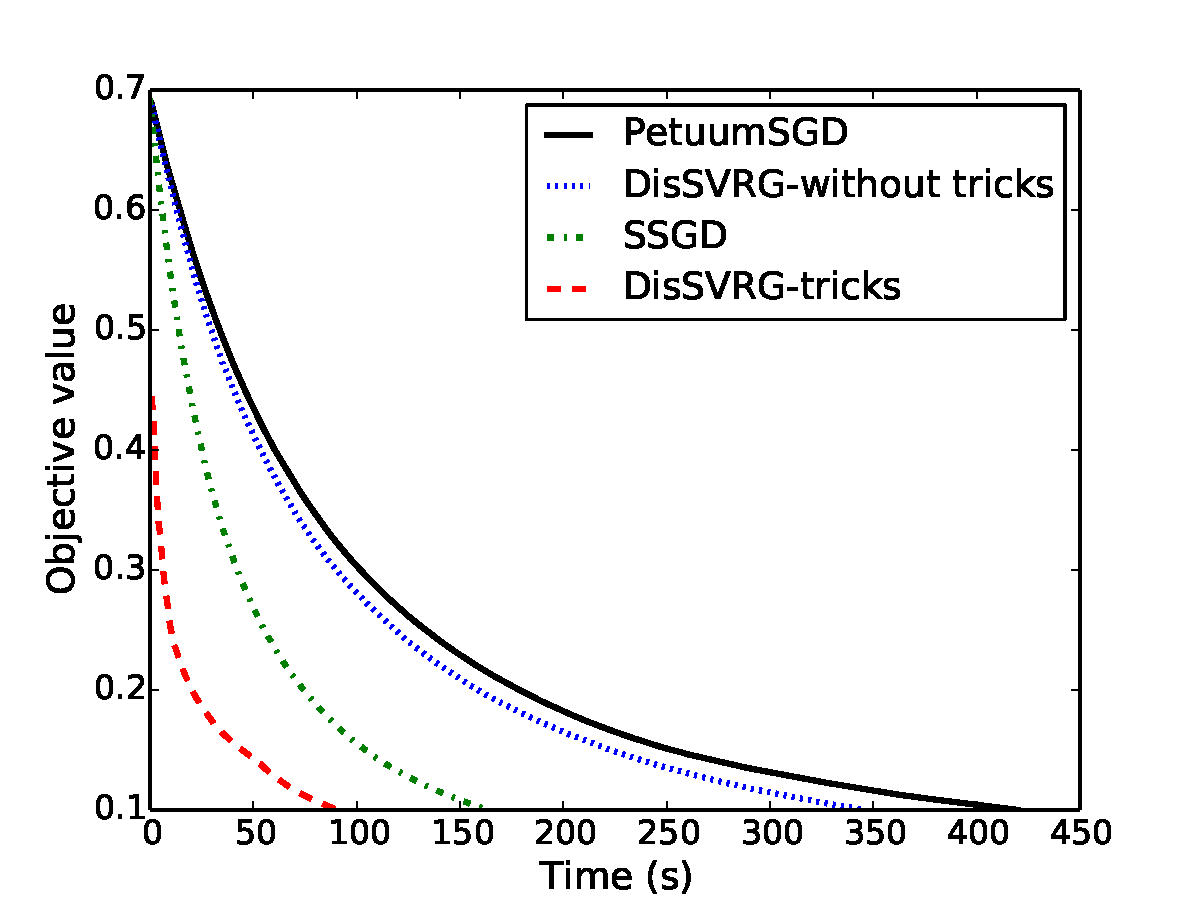
\includegraphics[width=0.49\columnwidth]{figures/evaluation1_converage}}
\subfigure[\emph{dna}]{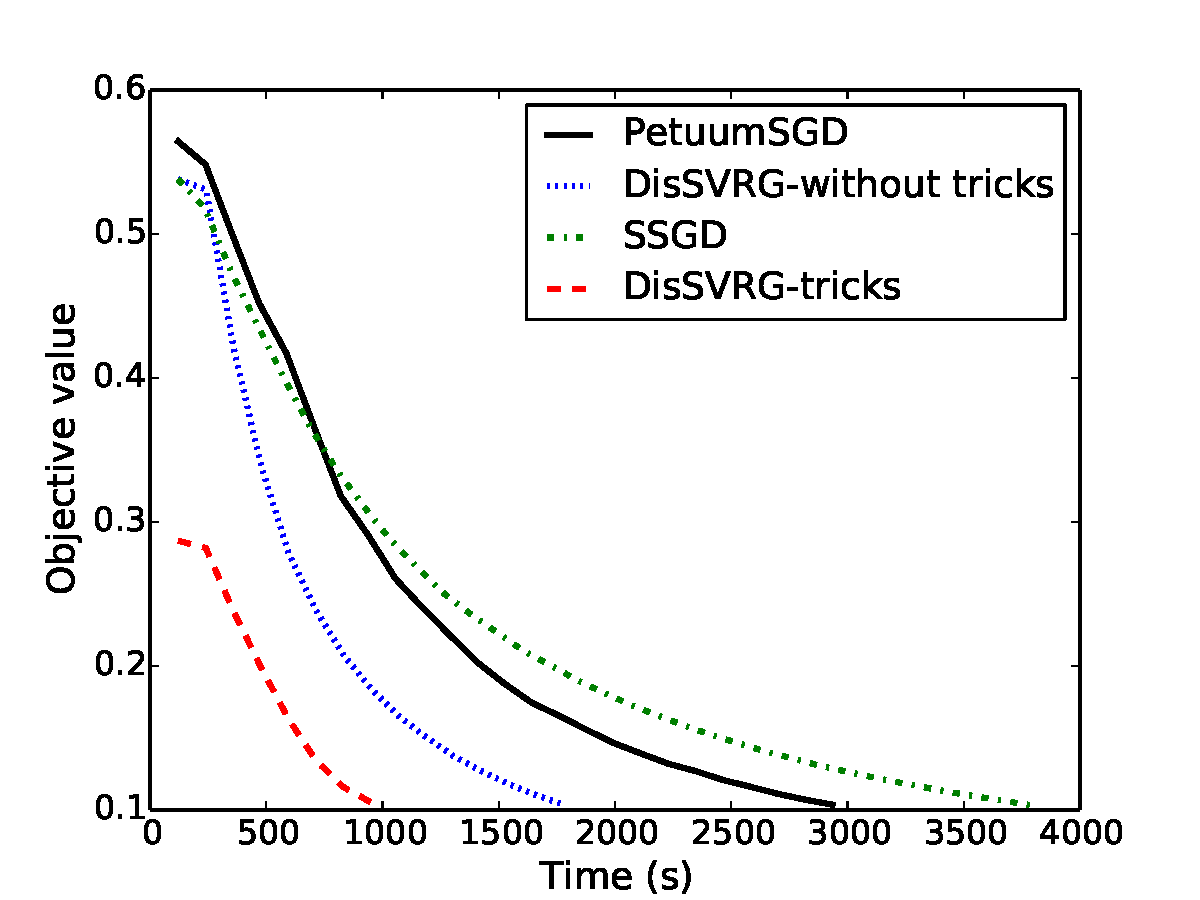
\includegraphics[width=0.49\columnwidth]{figures/evaluation1_dna_converage}}
\caption{The performance of the convergence is compared by using $32$ computing nodes.}
\label{figure_evaluation1_convergence}
\end{figure*}

\subsection{Speedup}
As illustrated in Fig. \ref{figure_evaluation2_speedup}, we compare the convergence performance of DisSVRG by varying the number of workers in a cluster. It is obvious that DisSVRG converges fast with a large number of workers. During the iterations, the more workers are used to update the local parameters, the more newly learned parameters will be aggregated with the global parameters. After that, the global parameters which contains the newly learned updates of parameters will be shared with other workers for the next iteration, thus accelerating the convergence of other workers. In specific, DisSVRG obtains appriximately linear speedup when varying the number of workers. For instance, DisSVRG gains $19\times$ speedup on the dataset \emph{YearPredictionMSD} when using $32$ workers. DisSVRG even keeps the linear speedup when using $128$ workers for the dataset \emph{dna}. The approximately linear speedup mainly benefits from the asynchronous communication protocol and the variance reduction technique. The asynchronous communication protocol relaxes the bound of the synchronization among workers, which alleviates the straggler problem, and thus decreases the wait time. The variance reduction technique reduces the variance of SGD, and keeps DisSVRG converging at a constant rate.

\begin{figure*}
\centering
\subfigure[\emph{YearPredictionMSD}]{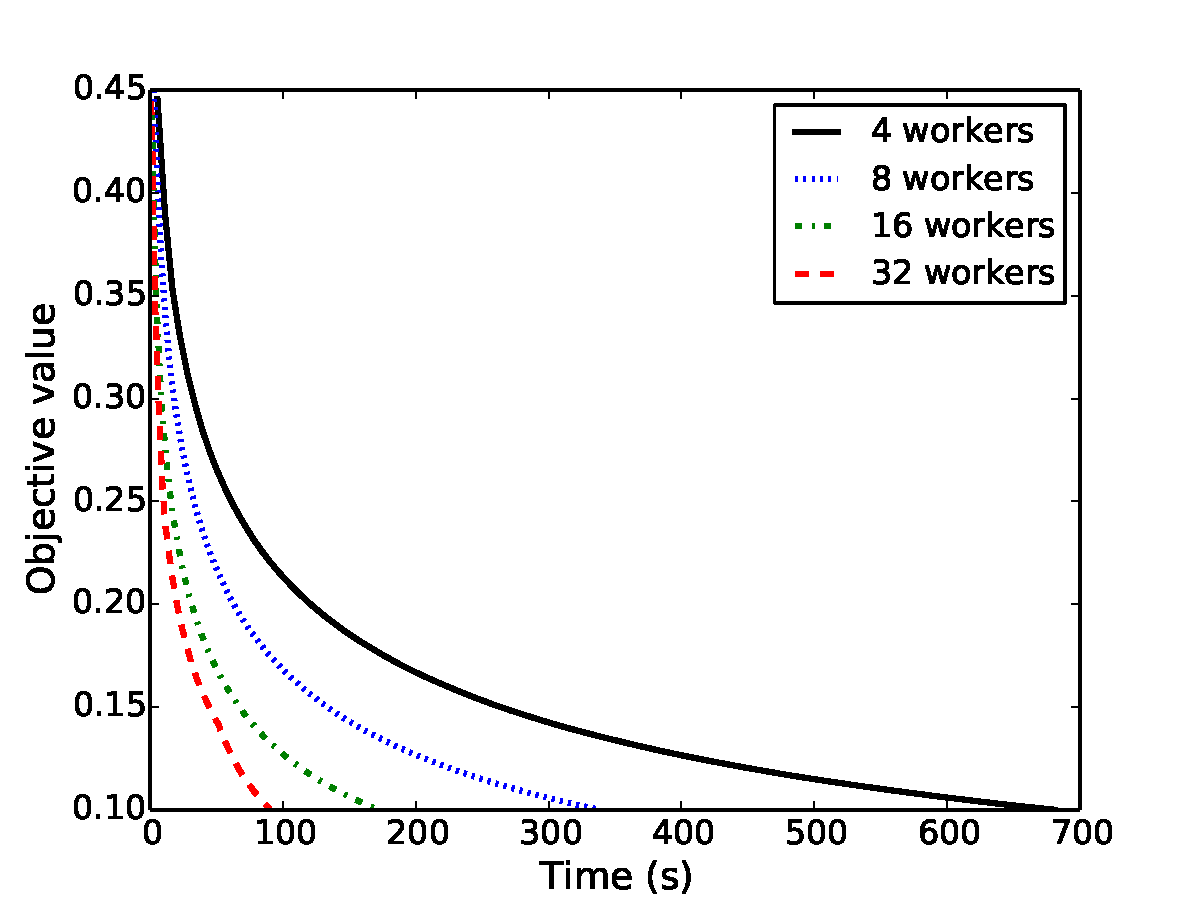
\includegraphics[width=0.49\columnwidth]{figures/evaluation2_speedup}}
\subfigure[\emph{dna}]{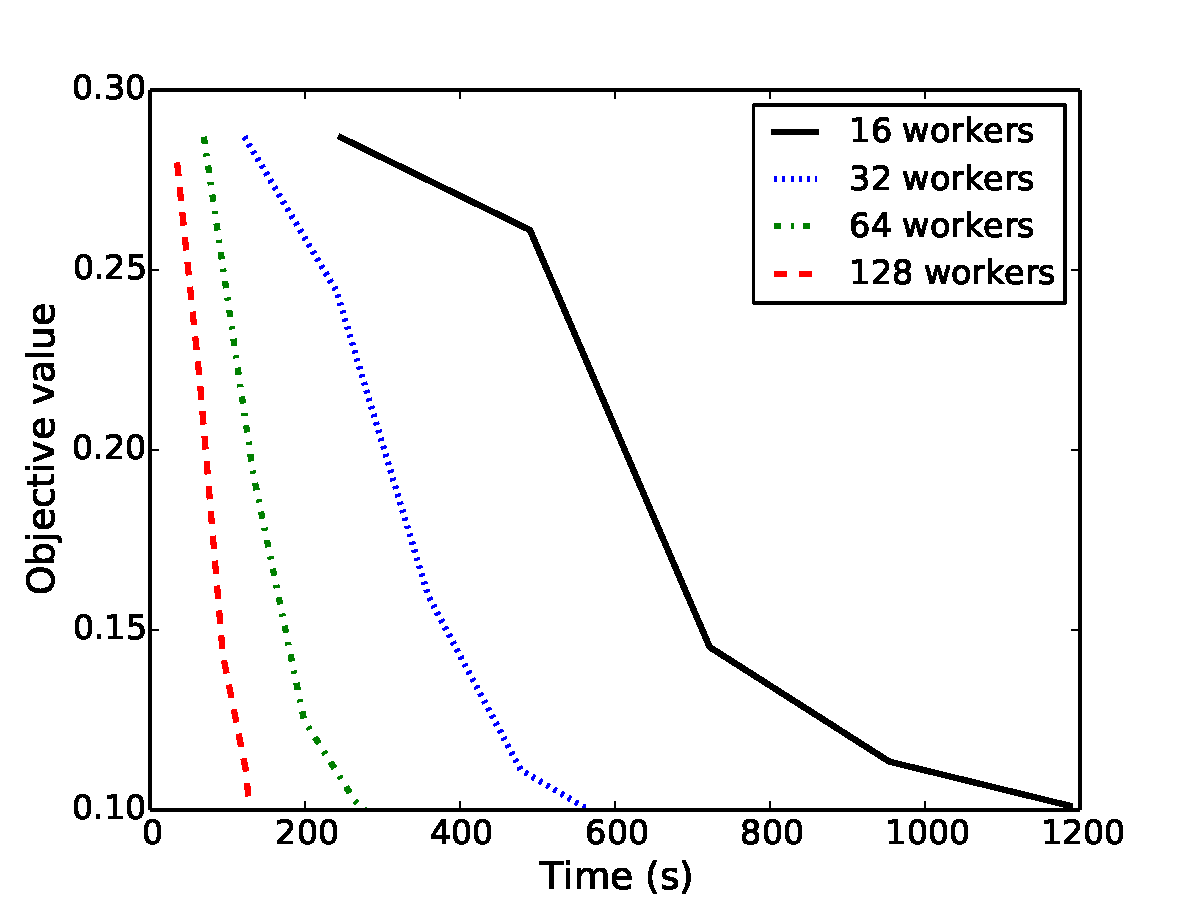
\includegraphics[width=0.49\columnwidth]{figures/evaluation2_speedup_dna}}
\caption{DisSVRG obtains almost linear speedup when varying the number of workers.}
\label{figure_evaluation2_speedup}
\end{figure*}

\subsection{Wait time}
As shown in Fig. \ref{figure_evaluation3_delay}, we evaluate the average time consumption of DisSVRG by varying the value of the delay $\tau$. It is obvious when the delay $\tau$ is small, the average wait time is large. A small delay means a tight bound among workers, which usually leads to the wait time for the fast workers due to the asynchronous communication protocol. For example, when the delay is set to be $0$, all the workers should be synchronized for each iteration, thus waiting the longest time. It is worth noting that the wait time decreases sharply when the delay becomes large. We conclude that a relax bound is effective to reduce the average wait time. Meanwhile, the average computing time will increase slightly with a relax bound of the delay. Although the fast workers have more freedom to conduct the iterations with the relax bound of the delay, the slow workers cannot obtain the newly learned parameters from the fast workers within the large delay. The slow workers thus cannot  benefit from the fast peers. In a nutshell, the delay should not be identified either too small or too large. It is a tradeoff between the wait time and the computing time for the workers. Generally, the delay should be set to minimize the total time consumption of DisSVRG. In our evaluation tests, the delay $\tau$ should be set to be  $200$ for the dataset \emph{YearPredictionMSD}, and $50$ for the dataset \emph{dna}.

\begin{figure*}
\centering
\subfigure[\emph{YearPredictionMSD}]{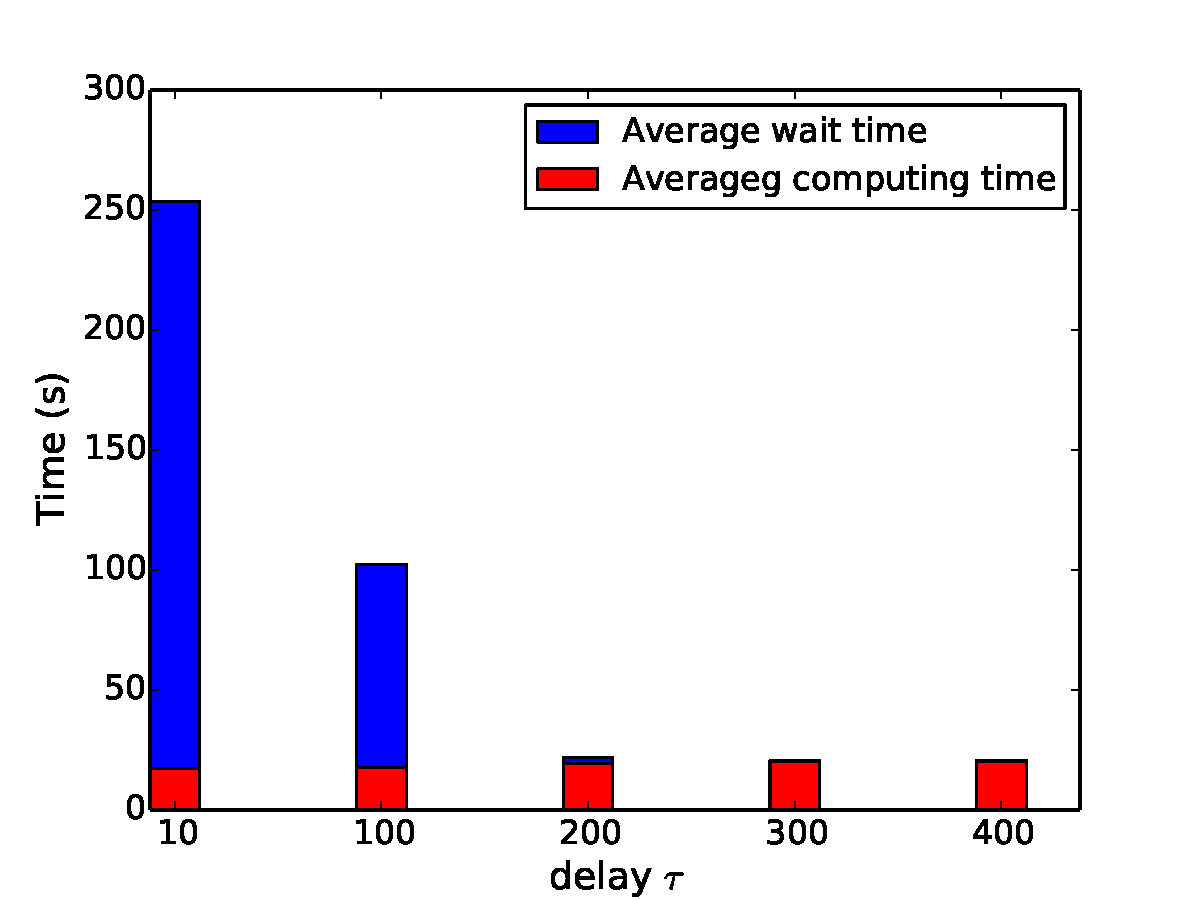
\includegraphics[width=0.49\columnwidth]{figures/evaluation3_delay}}
\subfigure[\emph{dna}]{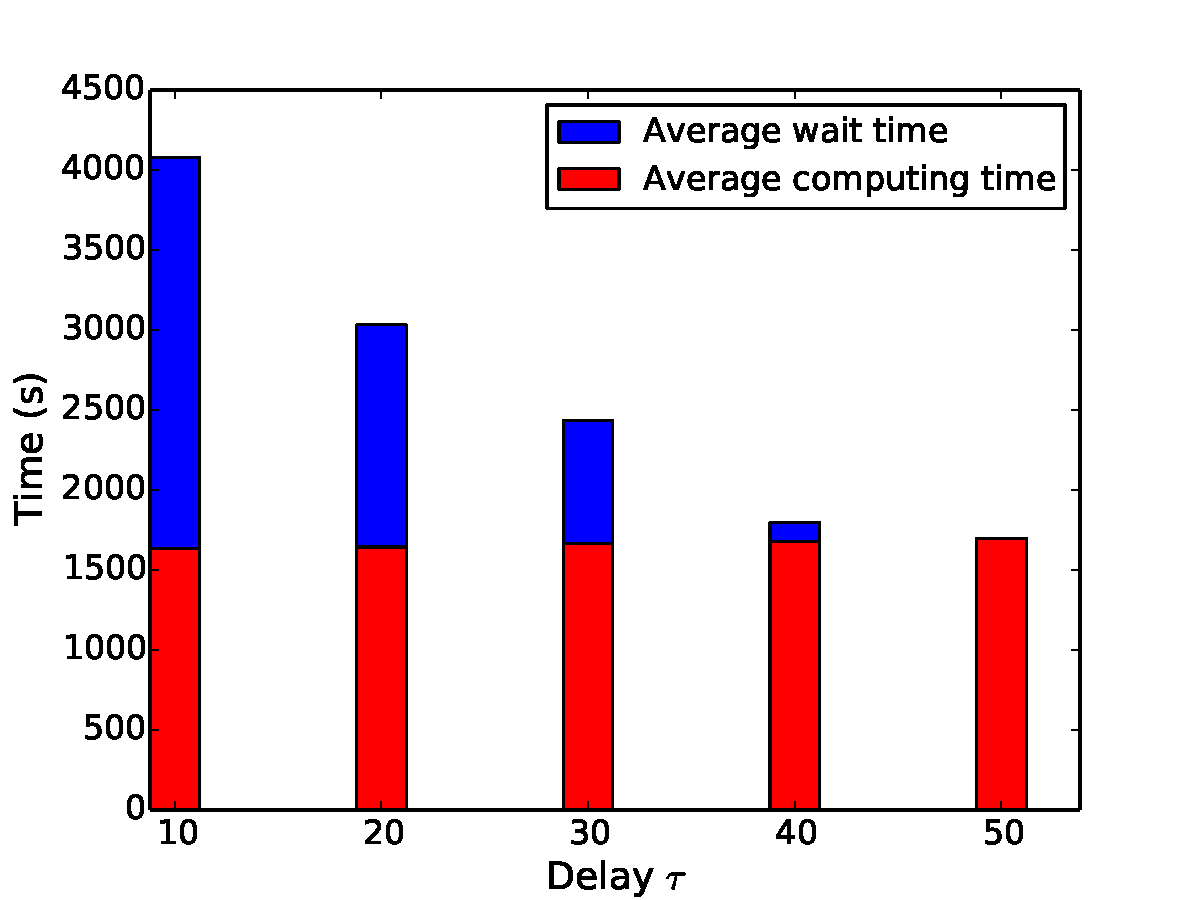
\includegraphics[width=0.49\columnwidth]{figures/evaluation3_delay_dna}}
\caption{The time consumption is compared by varying the delay $\tau$ for $128$ workers.}
\label{figure_evaluation3_delay}
\end{figure*}

\section{Conclusion}
\label{conclusion}
Distributed SGD is an effective way to solve the large scale learning problems. In this paper, we propose a version of distributed SGD named DisSVRG with combing the asynchronous communication protocol and the variance reduction technique. Exploiting the properties of the loss function, DisSVRG is optimized by using a learning rate with the acceleration factor. Additionally, in order to reduce the wait time caused by the straggler problem, we propose an adaptive sampling strategy during the iterations. The adaptive sampling strategy gives the slow workers a chance to catch up with the fast peers during iterations, thus alleviating the straggler problem. Extensive empirical studies show that DisSVRG converges faster than the state-of-the-art version of SGD, and can gain approximately linear speedup in a cluster.

\section*{Acknowledgment}
We thank the National Supercomputing Center in Changsha for providing \emph{Tianhe-1} supercomputer as our experiment platform. This work was supported by the National Natural Science Foundation of China (Project NO. 61672528, 61170287, 61232016, 61303189 and 31501073).

\section*{References}
\bibliographystyle{elsarticle-num}
\bibliography{reference}

\end{document}
